\chapter{Le \emph{framework} <<\emph{Mechanics}, \emph{Dynamics}, \emph{Aesthetics}>> (MDA)}
\label{chap.MDA}

\gt{Pas trop clair le d\'ebut!?}

La conception de jeux est le processus de réflexion nécessaire à la création d'un jeu.
C'est l'évolution que subit le jeu depuis une idée initiale jusqu'à sa réalisation finale.
De nombreuses étapes permettent de modéliser et formaliser tous les aspects du jeu pour le mener à sa version jouable : 
la mise en place du cadre spatio-temporel dans lequel le joueur évoluera, les règles qu'il devra suivre pour avancer, les éléments graphiques qu'il rencontrera. Tout cela est défini lors de la conception. 

Un jeu vidéo est cependant difficile à concevoir et, surtout, à documenter.
Un logiciel classique vise généralement \`a répondre à un besoin précis identifié et demandé par les utilisateurs.
Le logiciel est donc une réponse à une problématique et son utilisation est logique si le logiciel répond au besoin énoncé.
%
Par contre, un jeu vidéo doit créer le besoin chez un utilisateur, qui n'a pas de besoins liés à son utilisation.
Il doit proposer un but au joueur, lui donner l'envie de continuer à l'utiliser et doit générer des émotions pour être apprécié, car il ne vise pas \`a r\'esoudre une problématique.

Il est compliqué de définir une méthode précise pour décrire une émotion ainsi que les moyens à mettre en place pour parvenir à la générer.
Le \emph{framework} \glsfirst{mda} tente de définir une structure pour accompagner un \emph{game designer} durant les étapes de documentation d'un jeu.
MDA essaie d'apporter une solution en apportant une catégorisation des émotions et des approches et techniques pour parvenir à les générer.


\section{Le jeu : un échange entre \emph{game designer} et joueur}


\gt{Ne pas oublier: mettre un espace ins\'ecable --- tilde --- avant cite et avant ref!}


\begin{figure}
    \begin{center}
    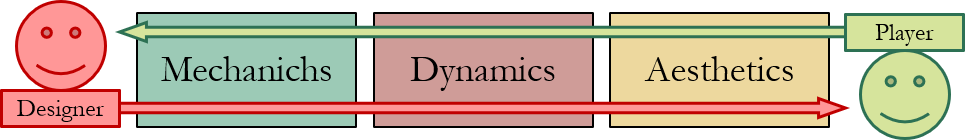
\includegraphics[width=14cm]{10_img/chap3/mda.png} 
    \caption{Les trois parties du \emph{framework} MDA~\cite{MDA_formal}.}
    \label{fig:mda}
    \end{center}
\end{figure}

Un \emph{game designer} cr\'ee un jeu dans le but de générer une expérience de jeu. 
Cependant, l'utilisation que le joueur fera du produit fini est difficile \`a pr\'evoir, comme
le d\'ecrivent Hunicke, LeBlanc et Zubek~\cite{MDA_formal}, qui découpent un jeu en trois aspects distincts : les règles, le système et le <<~fun~>>. 
Ces trois aspects sont à l'origine des trois parties du \emph{framework} MDA, tel qu'illustré dans la Figure~\ref{fig:mda}, que nous expliquons plus en d\'etail dans les sections qui suivent.


%MDA: A Formal Approach to Game Design and Game Research Robin Hunicke, Marc LeBlanc, Robert Zubek
%A better recipe for game jams: using the Mechanics Dynamics Aesthetics framework for planning Paris Buttfield-Addison,Jon Manning,Tim Nugent
%\Design, Dynamics, Experience (DDE): An Advancement of the MDA Framework for Game Design
\section{\emph{Mechanics}}

\label{mechanics.sect}

\gt{Malgr\'e le <<s>> final, <<mechanics>> est singulier --- comme la
m\'ecanique quantique.  Au singulier, <<mechanic>> d\'enote un
m\'ecanicien~:
\url{https://www.merriam-webster.com/dictionary/dynamics}. Idem pour
les autres aspects de MDA.}

\gt{Je ne comprends pas la 2e phrase, qui ne dit pas grand chose je
trouve: <<Les \'elements [\ldots[ plus pr\'ecis\'ement. J'ai tent\'e de reformuler.}

L'aspect \emph{Mechanics} d'un jeu est compos\'e de tous les éléments du jeu associ\'es \`a la représentation des données et des algorithmes. 
Les éléments de \emph{Mechanics} sont class\'es en diverses catégories, qui permettent de les définir plus précisément. 
Ces catégories peuvent comprendre des attributs et des spécificités qui sont appliquées aux divers éléments de chaque catégorie.

La \emph{Mechanics} comprend également les actions, comportements et mécanismes de contrôles mis à disposition du joueur. 
Cela peut correspondre aux mouvements d'un personnages, aux actions possibles sur des objets ou aux interactions entre les objets. Les règles sont aussi définies dans les mécaniques.


\section{\emph{Dynamics}}

Les \'el\'ements de l'aspect \emph{Dynamics} repr\'esentent les conséquences des \'el\'ements de \emph{Mechanics}. 
Ils décrivent le comportement de l'exécution de la \emph{Mechanics}, lorsqu'ils seront effectivement utilisées par le joueur~\cite{GAMA_MDA}. 
Ces \'el\'ements de \emph{Dynamics} sont importants à prévoir car ce sont eux qui permettront l'évolution du joueur dans le jeu.

Afin de définir la \emph{Dynamics}, il est possible d'analyser d'autres jeux (de même genre ou d'opus précédents); il est aussi possible d'effectuer des analyses statistiques sur les habitudes de jeu des joueurs, d'étudier leur psychologie afin de prévoir leur \emph{gameplay} et en jouant sur leurs émotions.


\section{\emph{Aesthetics}}
Les \'el\'ements de l'aspect \emph{Aesthetics} sont, selon Hunicke, LeBlanc et Zubek~\cite{MDA_formal}, <<~ce qui rend le jeu \emph{<<fun>>}~>>. 
Ce sont toutes les émotions générées par le jeu et transmises au joueur par l'interm\'ediaire de la mécanique de jeu, des sons ou des graphismes. Hunicke, Leblanc et Zubek classifient ces \'el\'ements en huit catégories :
\begin{itemize}
    \item Sensation : le jeu comme plaisir des sens.
    \item Fantaisie : le jeu comme imaginaire.
    \item Narration : le jeu comme situation dramatique.
    \item D\'efi : le jeu comme parcours d'obstacles.
    \item Communauté : le jeu comme réseau social.
    \item Découverte : le jeu comme territoire inexploré.
    \item Expression : le jeu comme découverte de soi-même.
    \item Soumission : le jeu comme passe-temps.
\end{itemize}

\gt{Les tildes (espaces ins\'ecables) sont important si tu utilises
guilletmotleft/right! Je trouve plus simple d'utiliser <<...>>, ce qui
donne la m\^eme chose sur ma machine. Et sur Overleaf, \c{c}a donne le
bon r\'esultat ou pas?}

Le jeu final peut contenir une ou plusieurs catégories de <<fun>> et l'ensemble de l'expérience du joueur repose sur ces \'el\'ements d'\emph{Aesthetics}. 
Cette dernière partie du \emph{game design} est si importante qu'il est possible de concevoir et développer le jeu en ayant au préalable sélectionné un certain nombre de ces catégories et en les considérant comme objectifs à atteindre.




\section{Des évolutions du \emph{framework} MDA}

Le MDA permet de modéliser la conception du jeu vidéo en séparant trois aspects cl\'es d'un jeu : les éléments de \emph{Mechanics}, de \emph{Dynamics} et d'\emph{Aesthetics}.
Cependant, de nombreux auteurs critiquent MDA car certains genres de jeu ou certaines mécaniques de \emph{gameplay} sont exclus de ce \emph{framework}.
%
D'autres \emph{frameworks} ont donc été proposés.
%
Par exemple, les \emph{frameworks} <<~\emph{Design, Play, Experience}~>> (DPE) (Sect.~\ref{sect.MDA_DPE}) --- qui cherche à intégrer les jeux reposant uniquement sur l'histoire, les jeux sérieux ou les outils d'apprentissage ludique ---
%
et <<~\emph{Design, Dynamics, Experience}~>> (DDE) (Sect.~\ref{sect.MDA_DDE}) --- qui avance que MDA néglige certains aspects du design de jeux vidéos en se concentrant trop sur les éléments de \emph{Mechanics}.

\gt{En quelques mots, en guise <<d'introduction>> \`a cette
section, il faudrait indiquer certaines limitation de MDA, pour
motiver pourquoi d'autres frameworks ont \'et\'e propos\'es.}


\subsection{Le \emph{framework} <<\emph{Design, Play, Experience}>> (DPE)}
%ARTCILE The Design, Play, and Experience Framework, Brian M. Winn
\label{sect.MDA_DPE}

\begin{figure}[H]
    \centering
    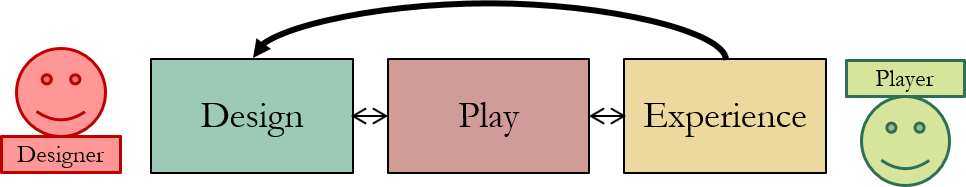
\includegraphics[width=10cm]{10_img/chap3/dpe.png} 
    \caption{Les trois parties du \emph{framework} DPE~\cite{Winn2011}.}
    \label{fig.dpe}
\end{figure}

Le \gls{dpe}, illustr\'e \`a la figure~\ref{fig.dpe}, est un \emph{framework} reposant sur les mêmes principes que MDA. 
Plus sp\'ecifiquement, des modifications sont appliquées au MDA afin d'étendre ses capacités de design pour les jeux sérieux. 
Ainsi, DPE étend MDA afin d'y intégrer les notions d'apprentissage, de \emph{story telling}, de \emph{gameplay} et de composants technologiques spécifiques aux jeux sérieux. 
La figure~\ref{fig.dpe_extended} donne les différentes parties du DPE, telles que présentées par Winn~\cite{Winn2011}.


\begin{figure}
    \centering
    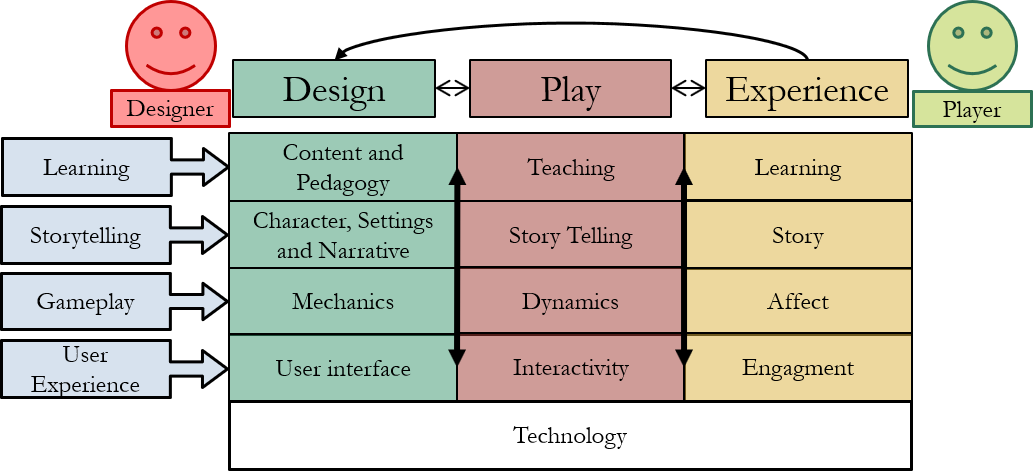
\includegraphics[width=14cm]{10_img/chap3/dpe_extended.png} 
    \caption{Les d\'etails du \emph{framework} DPE~\cite{Winn2011}.}
    \label{fig.dpe_extended}
\end{figure}


\begin{figure}
    \centering
    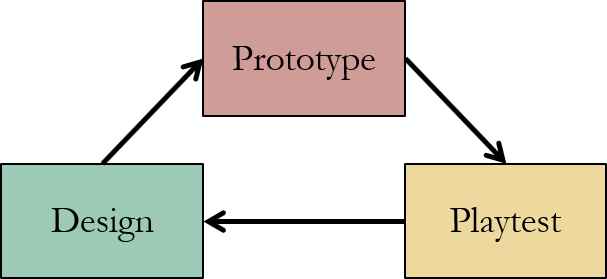
\includegraphics[width=8cm]{10_img/chap3/iteration_prototype.png} 
    \caption{Le processus de design itératif associ\'e \`a DPE~\cite{Winn2011}.}
    \label{fig.dpe_iteratif}
\end{figure}


Dans le \emph{framework} DPE, le \emph{game designer} a le contrôle direct sur l'ensemble des catégories. 
Notamment, le \emph{game designer} définit explicitement des objectifs d'\emph{Experience}. 
C'est ce qui est représenté, dans la figure~\ref{fig.dpe_extended}, par la flèche entre allant d'\emph{Experience} vers \emph{Design}. 
Cette flèche représente également le processus itératif du design décrit par Salen et Zimmermann~\cite{Salen2013}, tel qu'illustr\'e \`a la figure~\ref{fig.dpe_iteratif}. 
La conception permet de produire un prototype, et l'expérience sur ce prototype permet de modifier le design afin que l'\emph{Experience} corresponde aux attentes du \emph{game designer}.




\subsection{Le \emph{framework} <<~\emph{Design, Dynamics, Experience}~>> (DDE)}
\label{sect.MDA_DDE}
%ARTICLE DDE Design, Dynamics, Experience (DDE): An Advancement of the MDA framework for Game Design Wolfgang

\begin{figure}
    \begin{center}
    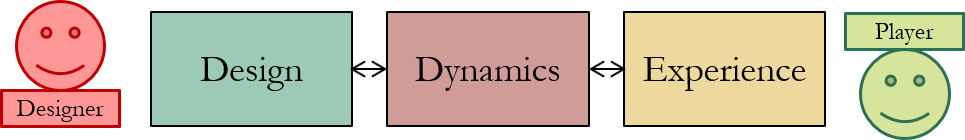
\includegraphics[width=10cm]{10_img/chap3/dde.png} 
    \caption{Les \'el\'ements du \emph{framework} DDE~\cite{DDE}.}
    \label{fig.dde}
    \end{center}
\end{figure}

\begin{figure}
    \begin{center}
    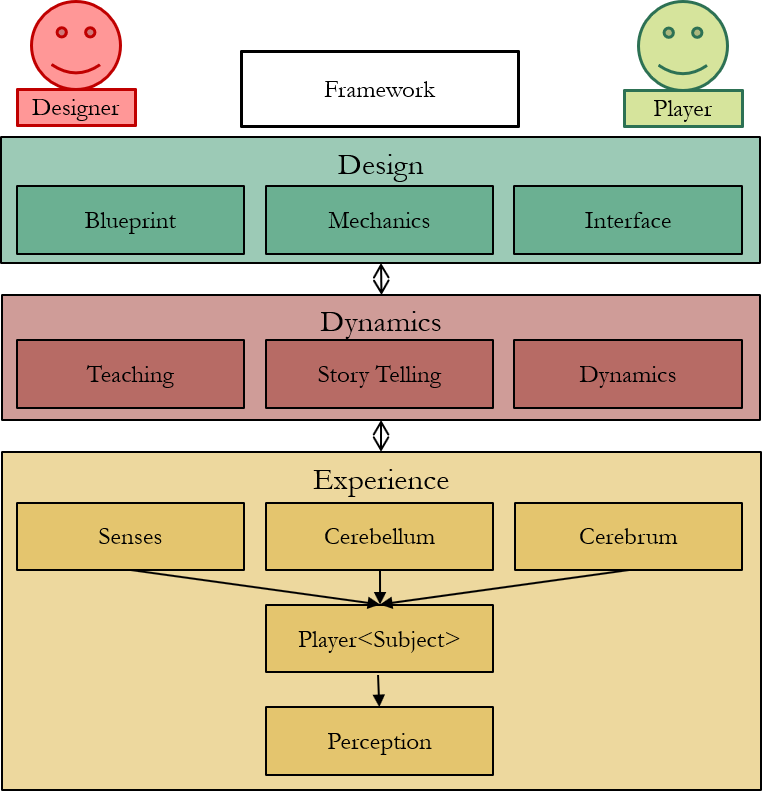
\includegraphics[width=13cm]{10_img/chap3/dde_extended_modif.png} 
    \caption{Les d\'etails du \emph{framework} DDE~\cite{DDE}.}
    \label{fig.dde_extended}
    \end{center}
\end{figure}

%GAMASUTRA From MDA to DDE, Wolfgang Walk
Le framework \gls{dde}, illustr\'e \`a la figure~\ref{fig.dde}, a \'et\'e propos\'e par Walk \emph{et~al.}~\cite{DDE}. 
Ils apportent une vision critique du \emph{framework} MDA et avancent que celui-ci néglige de nombreux aspects du design de jeux vidéos. 
Ils estiment également que MDA se concentre trop sur l'aspect \emph{Mechanics} et ne permet donc pas de décrire tous les types de \emph{gameplay} présents sur le marché. 
Ce focus sur l'aspect \emph{Mechanics} entraîne, selon Walk \emph{et~al.}, un manque de contrôle du \emph{game designer} sur les aspect \emph{Dynamics} et \emph{Aesthetics} qui ne font que découler de l'aspect \emph{Mechanics}
%
Walk \emph{et al.} effectuent donc un découpage différent et intègrent de nouvelles notions dans les catégories, tel qu'illustr\'e dans la figure~\ref{fig.dde_extended}.




\gt{J'ai mis des sous-sections non-numérotées, sinon c'est trop
profond comme numérotation et ça rend cela débalancé par rapport aux
autres sous-sections.}

\subsubsection*{\emph{Design}}

Les \'el\'ements associ\'es \`a l'aspect \emph{Design} sont les suivants~: 
    \begin{itemize}
\item \emph{Blueprint} : Partie du design qui concerne les concepts du monde du jeu : culture, religion, physique, ensembles de règles, styles artistiques, design narratif, design de personnages et design sonore, qui ensemble créent l'expérience esthétique.
\item \emph{Mechanics} : Toute chose créant le jeu, plus précisément le code. L'architecture du code, la prise en charge des entrées/sorties, la prise en charge des objets, l'implémentation des règles de jeu et l'interaction entre les objets, et tous les éléments reliés au code. Cela comprend donc tous les éléments que le joueur ne perçoit pas directement dans son utilisation du jeu.
\item Interface : Toutes les mécaniques qui ont pour but
    de communiquer le jeu au joueur. Les graphismes, les sons, les
    réactions et les interactions. Ces mécaniques peuvent aussi servir
    à effectuer une communication sous la forme
    Jeu~$\Rightarrow$~Joueur, Joueur~$\Rightarrow$~Jeu ou
    Jeu~$\Rightarrow$~Jeu. Cette partie comprend également les
    cinématiques, les textes affichés, et tout ce qu'il est possible
    de voir ou d'entendre dans le jeu.
\end{itemize}
%
\subsubsection*{\emph{Dynamics}} 

La catégorie \emph{Dynamics} de DDE correspond à celle de MDA, mais elle classifie les interactions de manière à les rendre plus précises, d\'ecompos\'ees en trois sous-catégories: 


    \begin{itemize}
        \item \emph{Player} $\Leftrightarrow$ \emph{Game}
        \item \emph{Player} $\Leftrightarrow$ \emph{Player}
        \item \emph{Game} $\Leftrightarrow$ \emph{Game}
    \end{itemize}

\subsubsection*{\emph{Experience}}
    Dans le \emph{framework} MDA, la troisième partie est l'\emph{Aesthetics} : tout ce que le joueur sent et ressent lors de son activité et interaction avec le jeu. 
    La partie \emph{Exprience} du jeu étend l'\emph{Aesthetics} afin de prendre en considération que le joueur n'est pas uniquement la somme des émotions générées par le jeu. 
    Le joueur devient un élément avec une expérience déjà présente avant l'utilisation du jeu, ce qui peut modifier les émotions générées d'un joueur à l'autre. Une même couleur, un même son ou une même image peuvent générer différentes réactions de la part du joueur et la partie \emph{Experience} de DDE essaie de prendre cela en compte.
    \begin{itemize}
        \item \emph{Senses}: expérience sensorielle du joueur du début à la fin du jeu.
        \item \emph{Cerebellum} : les émotions ressenties par le joueur.
        \item \emph{Cerebrum} : les d\'efis intellectuels et les décisions prises par le joueur.
        \item \emph{Player<Subject>} : la partie que le designer ne peut pas contrôler. Il peut se baser sur les trois premières catégories afin de prévoir certaines réponses spécifiques du joueur. N'ayant aucun contrôle sur celles-ci, le designer ne peut qu'estimer la réaction du joueur en fonction d'objectifs et de logiques psychologiques pour l'amener à la réaction souhaitée.
        \item \emph{Perception} : ce que ressent réellement le joueur en fonction des trois premières catégories et de sa propre expérience et personnalité en tant que joueur. Cela comprendra son \emph{gameplay}, le type de d\'efi qu'il perçoit, l'amusement qu'il ressent, la beauté qu'il perçoit, l'écho que génère l'histoire en lui, etc.
    \end{itemize}


%GAMASUTRA Revisiting the MDA framework, Luiz Claudio Silveira Duarte
\subsection{Une autre limite du \emph{framework} MDA}
Dans une critique du \emph{framework} MDA, Duarte~\cite{GAMA_MDA} met de l'avant les difficultés  rencontr\'ees à représenter, \`a l'aide de MDA, des jeux qui ne soient pas des jeux vidéos. 
Duarte explique que les règles d'un jeu vidéo sont souvent implicites au type de \emph{gameplay} ou genre de jeu vidéos. 
Cependant, dans le cadre des jeux de plateau, les règles ne peuvent pas être implicites et acquises par l'expérience. 
Elles doivent être explicites et explicables dans un manuel d'utilisation. 
Il fait l'analogie entre un jeu FPS --- \gls{fps} --- et un jeu d'échecs. Dans un FPS, un joueur sait à quoi s'attendre en fonction de son expérience du genre du jeu. 
Il saura o\`u trouver les éléments et saura comment faire usage de l'interface graphique qui lui est présentée. 
Cependant, un joueur se trouvant devant un jeu d'échecs pour la première fois ne pourra pas acquérir par l'exp\'erience les connaissances requises pour jouer~: les règles devront lui être expliquées à la base et l'expérience pourra lui apporter des aspects tactiques ou strat\'egiques du jeu.

\section{Conclusion}

\GT{Je trouvais cela un peu trop long de répéter tous ces éléments,
dans la conclusion, donc j'ai réduit. Et, surtout, pour Mechanics, il
faut insister sur les concepts plus que sur les règles, car c'est ce
que tu modélise avec ton profil et dans ton exemple --- pcq. sinon,
avec cette conclusion, un lecteur pourrait trouver que tu n'atteins
pas le bon objectif je trouve. Et il manquait aussi la transition vers
le prochain chapitre --- dernière phrase.}

Nous avons donc vu dans ce chapitre que le \emph{framework MDA} sépare la conception d'un jeu en trois aspects :
\begin{itemize}
    \item \emph{Mechanics} : Les \textbf{concepts} et les {règles}.
    \item \emph{Dynamics} : Le système et son \textbf{comportement} dynamique.
    \item \emph{Aesthetics} : Les \textbf{émotions} et le \textbf{\emph{<<fun>>}}.
\end{itemize}
Le but de cette recherche est d'apporter une aide à la rédaction d'un \emph{Game Design Document} qui commence par représenter les éléments présents dans le jeu et par identifier les principales interactions entre eux.
Dans notre recherche, nous avons donc décidé de nous concentrer sur la modélisation des éléments de \emph{Mechanics}, leur description ainsi que l'identification des interactions.
C'est ce que nous présentons,  dans le Chapitre~\ref{chap.game-genesis}, avec notre profil \emph{Game Genesis}.
%
Mais auparavant, nous devons introduire la notion de \emph{profil UML}.
